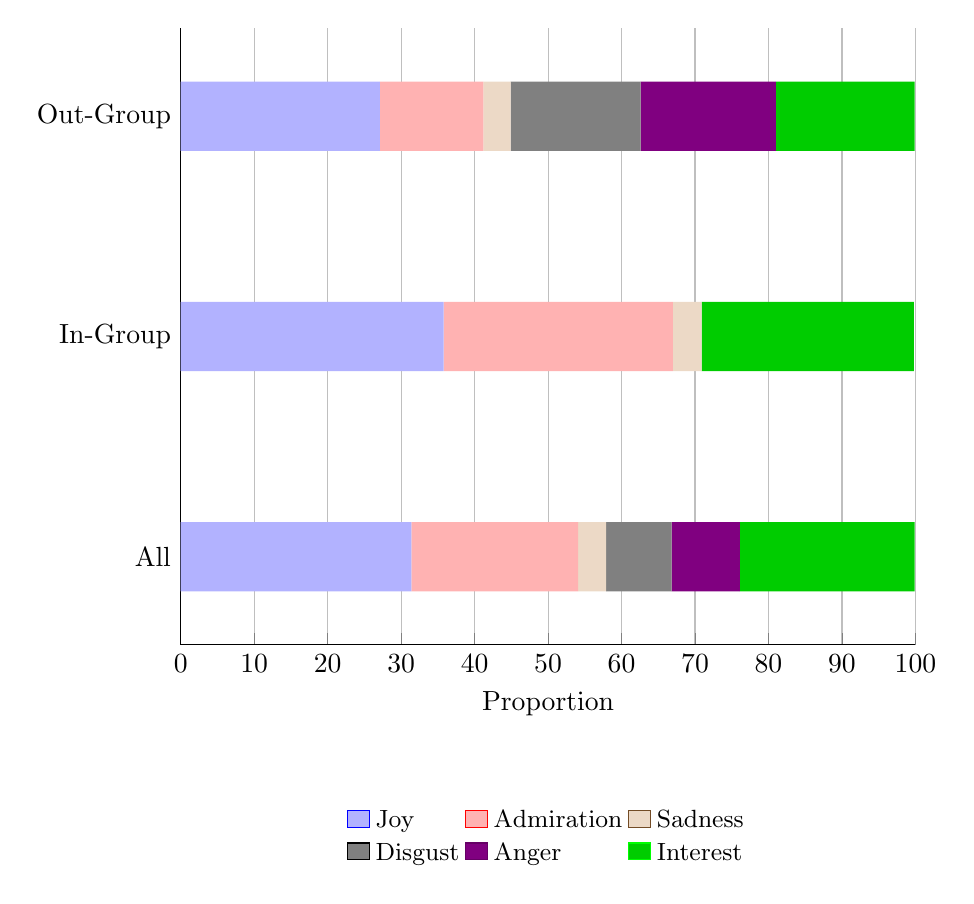
\begin{tikzpicture}
    \begin{axis}[
       xbar stacked,
       width  = 0.9\columnwidth,
       major y tick style = transparent,
       bar width=25pt,
       axis x line*=bottom,
       axis y line*=left,
       xmajorgrids = true,
       tick label style={/pgf/number format/assume math mode=true},
       xlabel = {Proportion},
       symbolic y coords={All,In-Group,Out-Group},
       ytick = data,
       extra y tick style={grid=none},
       xmin=0,
       xmax=100,
       scaled x ticks = false,
       enlarge y limits=0.2,
       legend cell align=left,
       legend style={
               draw=none,
               at={(0.5,-0.25)},
               anchor=north,
              text=black,
               font=\small,
               legend columns=3
               },
        % nodes near coords,
        % nodes near coords style={font=\tiny, text=white,/pgf/number format/assume math mode} 
   ]
       \addplot+[draw=none]
           coordinates {(31.4,All) (35.8,In-Group) (27.1,Out-Group)};

       \addplot+[draw=none]
           coordinates {(22.7,All) (31.2,In-Group) (14.1,Out-Group)};

       \addplot+[draw=none]
           coordinates {(3.8,All) (3.9,In-Group) (3.7,Out-Group)};
        
       \addplot+[draw=none]
           coordinates {(8.9,All) (0.0,In-Group) (17.7,Out-Group)};
        
       \addplot+[draw=none]
           coordinates {(9.3,All) (0.0,In-Group) (18.4,Out-Group)};
           
        \addplot+[draw=none]
           coordinates {(23.8,All) (28.9,In-Group) (18.9,Out-Group)};

       \legend{Joy, Admiration, Sadness, Disgust, Anger, Interest}
    \end{axis}
\end{tikzpicture}